\section[Cooling effectiveness]{Overall Effectiveness: Four Objectives, an Explicit Choice}
\label{sec:effectiveness}

\subsection{Performance, access, energy and annual cost}
Task 3 ranks useful service per kWh. Task 4 adds the operator's service and resource requirements. We compare
\begin{equation}
 \min_s\big(\overline R_s,\ X_s,\ E_{s,y},\ C_{s,y}\big),\qquad
 X_s=\frac{\sum_{z,k}x_{zk}b_k}{\sum_z A_z}.
\label{eq:effectiveness-vector}
\end{equation}
Here $\overline R_s$ is remaining SET excess; $b_k$ is equipment and maintenance clearance in m$^2$; and $X_s$ is the fraction of public service area lost, a \textit{visitor-access proxy}. Clear routes and exits remain layout requirements. Annual electricity $E_{s,y}$ and expenditure $C_{s,y}$ describe resource use and cost. Thermal relief is counted once; $\eta$ is not a fifth objective.

Using Table~\ref{tab:venue-inputs}, let $E_{s,y}=H_y\sum_{z,k}x_{zk}p_k$ and $\operatorname{CRF}=r(1+r)^L/[(1+r)^L-1]$. Then
\begin{equation}
 \begin{aligned}
 C_{s,y}&=\operatorname{CRF}\sum_{z,k}x_{zk}K_k+
             \sum_{z,k}x_{zk}M_k+\pi_eE_{s,y}+\pi_wV_{s,y},\\
 V_{s,y}&=\frac{3600H_y\lambda_w}{\rho_w}
          \sum_{z,k}x_{zk}\dot m_k(w_{e,k}-w_a).
 \end{aligned}
\label{eq:venue-cost}
\end{equation}
$K_k$ is capital cost (USD), $M_k$ annual maintenance (USD/year), $H_y$ hours/year and $\rho_w$ water density (kg/m$^3$). Thus $E_{s,y}$, $V_{s,y}$ and $C_{s,y}$ have units kWh/year, m$^3$/year and USD/year. Water is charged once per unit, including the make-up factor $\lambda_w$.

\subsection{An integer minimum-cost service policy}
An $\varepsilon$-constraint policy minimizes cost while setting explicit limits on the other outcomes:
\begin{equation}
 \begin{aligned}
 s^*={}&\arg\min_s C_{s,y},\qquad x_{zk}\in\mathbb Z_{\ge0},\\
 &\sum_k a_kx_{zk}\le A_z\quad(\text{every }z),\qquad q_s\ge0.80,\\
 &\frac{U_s}{\sum_z\mathcal H_z}\ge1.5^\circ\mathrm C,\qquad
 X_s\le0.035,\qquad E_{s,y}\le e_{\max}\sum_z A_z .
 \end{aligned}
\label{eq:effectiveness-selection}
\end{equation}
Here $a_k$ is the service footprint and $e_{\max}=30$ kWh/(m$^2\!\cdot$year). The mean-relief constraint is equivalent to a residual ceiling under each venue's fixed baseline. All coefficients are fixed by the physical model, giving nine integer variables in Fremont and three in Honolulu. The mixed-integer linear solver reports zero optimality gap for both nominal cases. This establishes the minimum cost over all feasible integer allocations under the stated policy.

\begin{table}[!ht]
\centering\small
\caption{Minimum annual cost under Eq.~\eqref{eq:effectiveness-selection}. Relief includes uncovered visitors; annual energy and cost are in kWh/year and USD/year.}
\label{tab:venue-decisions}
\begin{tabular}{@{}llrrrrr@{}}
\toprule
Venue & Plan & $q$ (\%) & Relief ($^\circ$C) & $X$ (\%) & $E_y$ & $C_y$\\
\midrule
Fremont & A266C16 & 81.79 & 1.5002 & 1.87 & 63,900 & 50,926\\
Honolulu & A1B1 & 83.33 & 1.5608 & 2.50 & 870 & 627\\
\bottomrule
\end{tabular}
\end{table}

One optimal Fremont assignment is $(116\mathrm A,\ 148\mathrm A+16\mathrm C,\ 2\mathrm A)$ across the three zones. It directs service toward high visitor density; the third zone receives only $1.68\%$ coverage. A requirement to serve every sector would need additional zonal coverage constraints. The selected plans leave mean SET excesses of $6.274^\circ$C and $3.902^\circ$C, respectively, so meeting the relief target does not imply thermal neutrality.

\begin{figure}[H]
\centering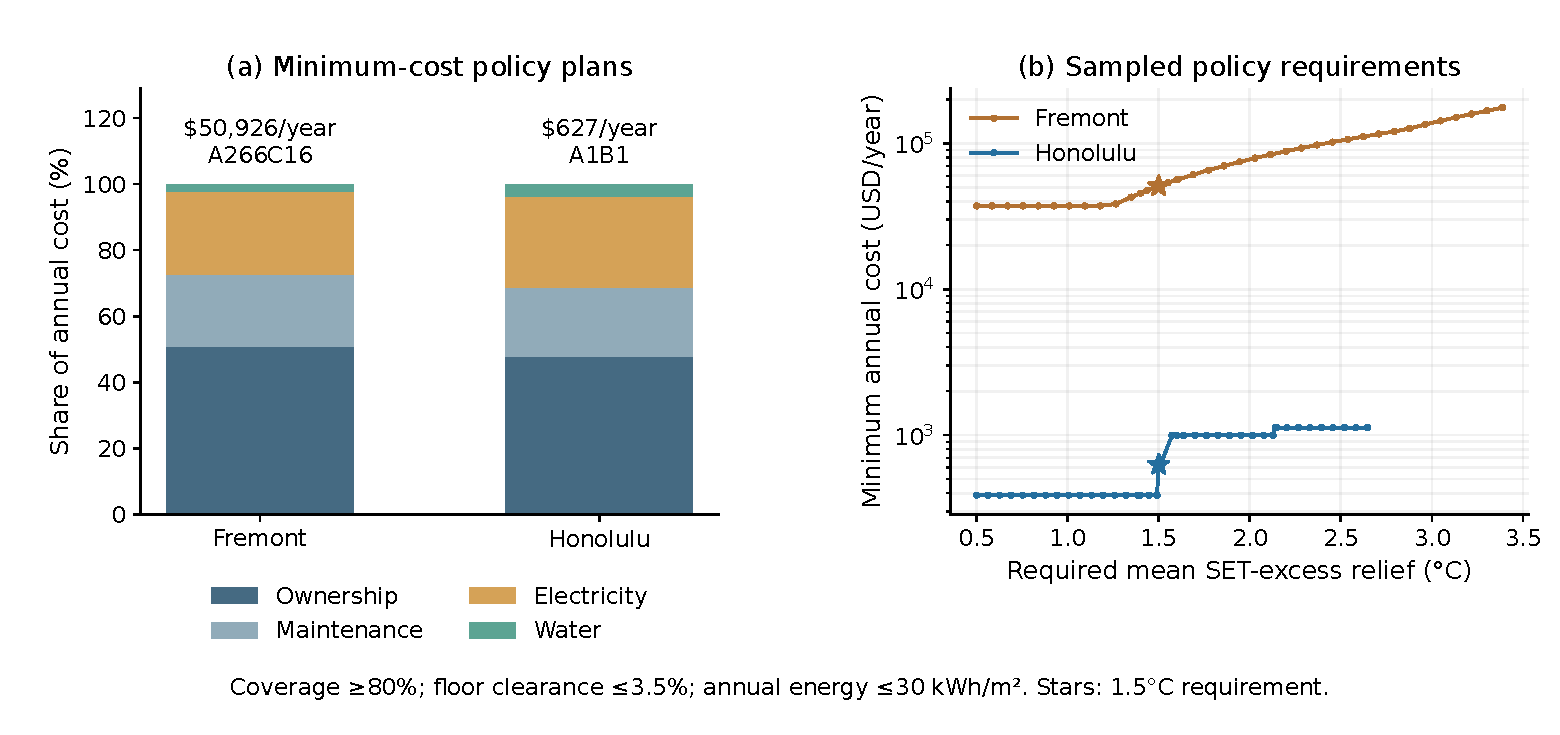
\includegraphics[width=\linewidth]{figures/28_effectiveness.pdf}
\caption{Annual cost composition and minimum cost versus required mean relief, with the other policy limits fixed. Stars mark the $1.5^\circ$C policy; the cost axis in the right panel is logarithmic. Integer choices create discrete transitions.}
\label{fig:venue-effectiveness}
\end{figure}

\begin{figure}[!ht]
\centering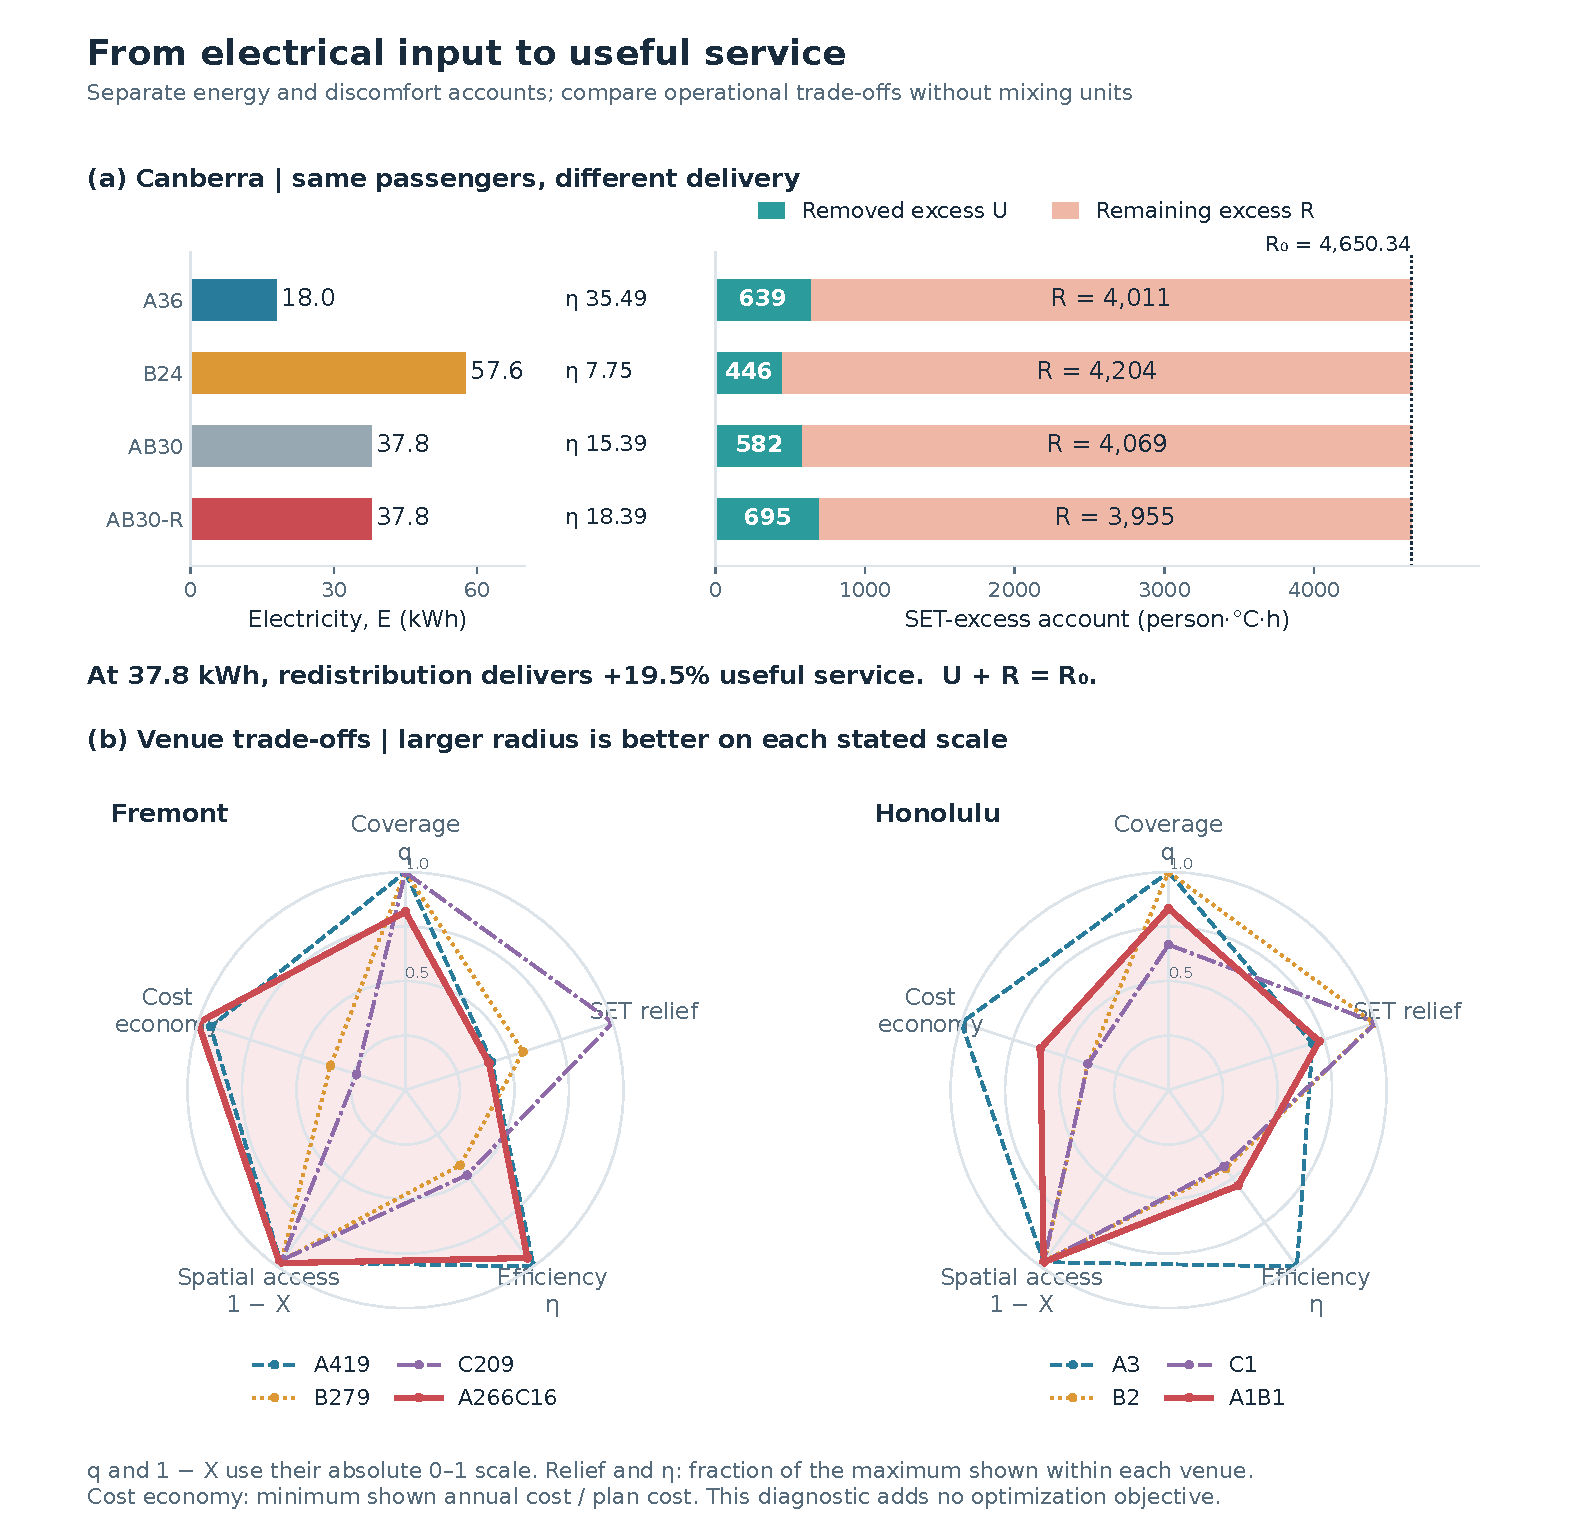
\includegraphics[width=\linewidth]{figures/36_energy_service_radar.pdf}
\caption{Separate accounts and operational trade-offs. (a) Electrical kWh and SET-excess person$\cdot{}^\circ$C$\cdot$h have distinct axes: $U+R=R_0$ is a service identity, not an energy partition. (b) Radar scales are stated in the figure; the selected mixed plans minimize policy cost, without dominating every pure-device indicator.}
\label{fig:service-radar}
\end{figure}

Figure~\ref{fig:service-radar} makes the distinction explicit: redistribution raises Canberra's useful service by $19.5\%$ at unchanged electricity. No measured motor-loss or ventilation-loss fractions are available, so SET service is not assigned a fictitious share of input kWh. The radar is a diagnostic of the existing solutions, not an additional optimization objective.

\subsection{Threshold sensitivity changes the recommendation}
In Honolulu, A3 provides full coverage and $1.4908^\circ$C relief: only $0.0092^\circ$C below the nominal target. Targets of $1.40$ or $1.49^\circ$C select A3 at USD 388/year; $1.50^\circ$C selects A1B1 at USD 627/year; $1.60^\circ$C selects B2 at USD 996/year. Thus the thermal service requirement controls the preferred configuration.

Across 243 price combinations, Honolulu retains A1B1 throughout; Fremont retains its nominal counts in 56 cases, while 69 select pure A398. Physical changes also matter: increasing Honolulu's background speed from $0.35$ to $0.8$ m/s selects A1C1 because the required benefit is measured above the improved natural-wind baseline. Reducing its queue area to $45$ m$^2$ makes the unchanged policy infeasible under full-footprint packing. Operators should establish service targets, usable area and delivery conditions before committing to a configuration.
